\section{Proposed Design}
\label{section:propeseddesign}

Before doing any implementation, we conducted some investigation into how Hadoop works, 
specifically how it assigns tasks initially and how they are reassigned during runtime.
These are important attributes to understand, because they contribute to uneven effective
workloads in a heterogeneous environment; that is, if two machines are assigned equal-sized
tasks, but one machine is twice as powerful as the other, it was effectively given half as
much work since it will complete it twice as fast as the other machine.

\subsection{Hadoop MapReduce Task Assignment}

We show the steps Hadoop MapReduce takes to carry out a job in \ref{fig:flow}. MapReduce 
works by taking map and reduce functions from the application (Wordcount for example), 
then configuring a \texttt{Job} object representing that application and its configuration.
Input data for the job is loaded into the Hadoop Distributed File System by the user. 
The job is then submitted to the \texttt{JobClient}, which subsequently calls the 
\texttt{getSplits} method to divide the input data to appropriate sizes to be sent out to
the MapReduce nodes. The \texttt{TaskTracker} on each slave node communicates with
the \texttt{JobTracker} on the master node to be assigned FileInput splits based on the
\texttt{TaskScheduler}. 

defining \texttt{FileInput} splits, and
assigned to nodes by the \texttt{TaskScheduler} via the \texttt{JobTracker}. 

\begin{figure}[ht!]
\centering
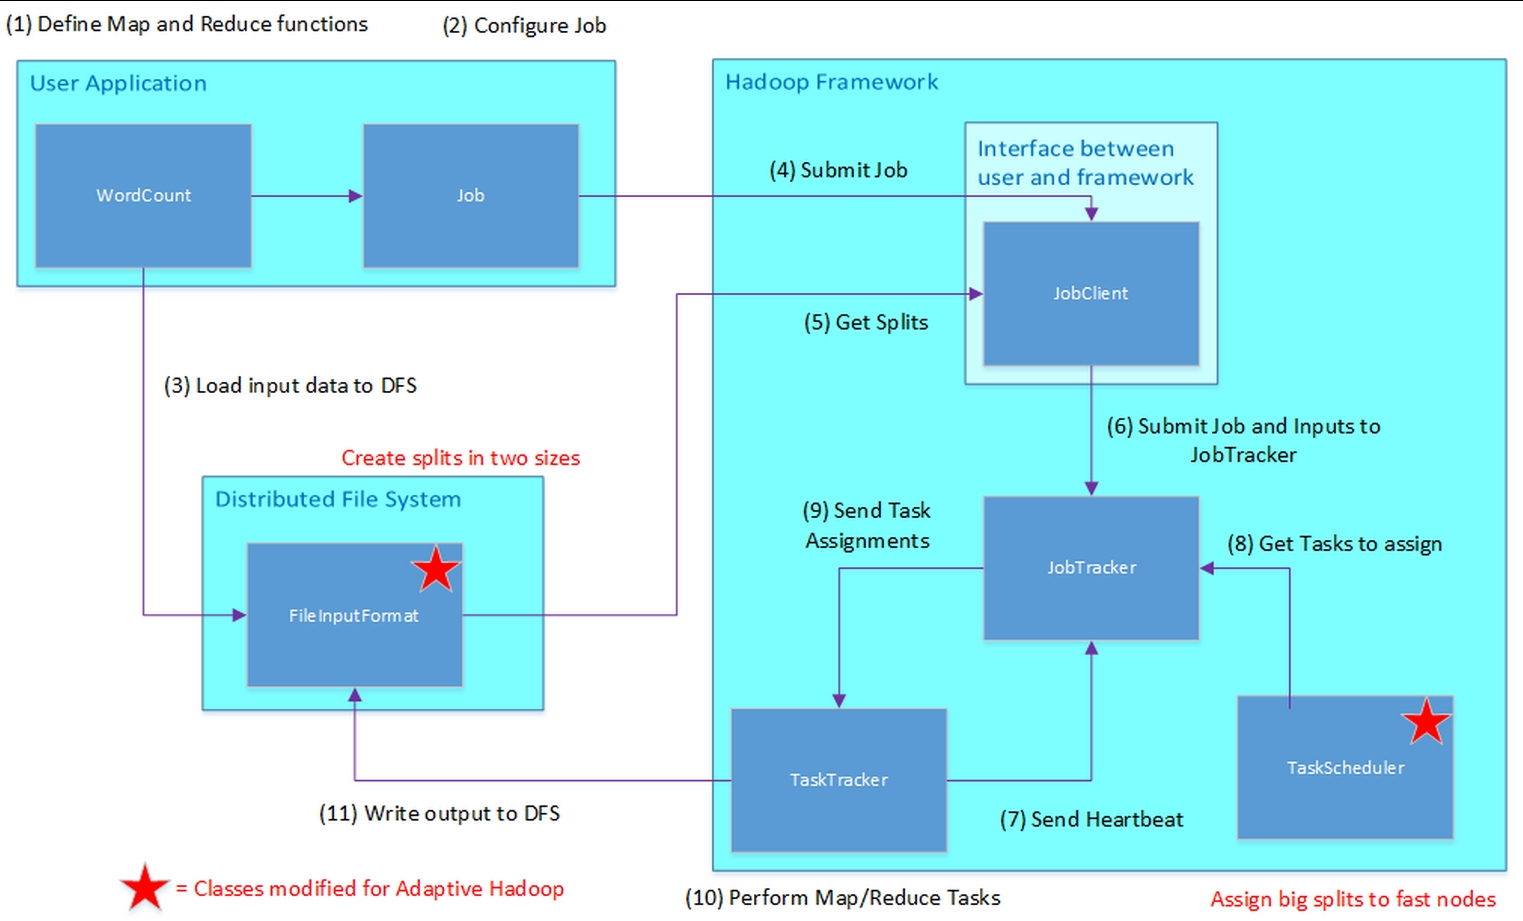
\includegraphics[width=90mm]{flow.jpg}
\caption{Workflow of a Hadoop MapReduce job}
\label{fig:flow}
\end{figure}

In standard Hadoop MapReduce, the Mapper divides up and distributes tasks to the workers.
Understanding this implementation is key to our research so that we can scale task sizes
to the computational capabilities of each MapReduce node. In Hadoop, a \texttt{JobConf}
object defines the configuration for each Mapper. By customizing this object per node,
we should be able to scale how much work a given node is given based on its capabilities.

A naive approach to scaling node task assignment would be to perform some basic performance
diagnostics during the task setup phase, and apply a simple weight coefficient to how much
work it should receive.

\subsection{Datacenter VM Interference}
\label{sec:interference}
In addition to hetergeneous machines, datacenters can also exhibit temporal heterogeneity.
VM performance depends on the behavior of other VMs on the same machine at any given time.
This means a VM on a machine with other, inactive VMs will initially be very performant;
but once the other VMs begin doing work the VM will experience performance degradation.
The variability of a VM's performance also depends on the abstraction layer between the VMs
and the physical hardware.

\subsection{Hadoop MapReduce Task Stealing}
The hardware interefence described in \ref{sec:interference} must be addressed dynamically
during runtime. An intuitive place to insert extra logic addressing this is during task
stealing.

In MapReduce jobs, each node is typically assigned a number of tasks. As some nodes 
complete their work ahead of schedule, they will steal tasks from other, backed-up,
nodes. If we modified the logic around which nodes to steal from, and how much work
to steal, we could help ensure all the tasks are finished closer to the same time.

